% !TeX root = main.tex

% ============================================================
% thesis-sync entry: 2026-07-19_inchworm-actuator-design-fem
% Type: design decision + numeric data (FEM optimization)
% Part of the INCHWORM ROBOT block (prior work, precedes the lizard sections).
% Insertable section block (no preamble).
% Requires in main.tex preamble: amsmath, graphicx, multirow, makecell.
%   -> add \usepackage{multirow} and \usepackage{makecell} to main.tex.
% ============================================================

\section{OMNIDIRECTIONAL BENDING ACTUATOR}
\label{sec:inchworm-actuator}

\subsection{Energy Model and Optimization Objective}

The total consumption of pneumatic energy per locomotion cycle,
$E_{cycle}$, can be estimated from the mechanical work required to
pressurize and evacuate the internal chambers. Modeling the energy of each
phase as the product of supplied pressure and internal volume, $E_{cycle}$
is expressed as:
\begin{equation}
	E_{cycle} = (P_{bend} V_{ch}) + 2(P_{vac} V_{cup}) + 3(P_{elong} V_{ch})
	\label{eqn:inchworm-energy}
\end{equation}
where $P_{bend}$ and $P_{elong}$ are the actuation pressures applied for
bending and elongation respectively, and $V_{ch}$ is the internal volume of
a single chamber. Anchoring energy relies on the vacuum pressure $P_{vac}$
and the evacuated suction volume $V_{cup}$. Passive venting during
relaxation and suction deactivation consumes zero energy.
Equation~(\ref{eqn:inchworm-energy}) assumes isobaric filling, providing a
conservative upper-bound estimate of the energy drawn from a
constant-pressure supply~\cite{Tolley2014Resilient}. Because the reduction
of the internal chamber volume is constrained by manufacturing limitations,
the optimization of energy consumption focused primarily on minimizing the
actuation pressure required to achieve a target bending angle.

\subsection{Actuator Geometry}

The silicone actuator body (Fig.~\ref{fig:inchworm-geometry}) consists of a
cylinder with three radially symmetric internal pneumatic chambers. Internal
walls converge at the central axis, dividing the interior into equal
$120^\circ$ sectors. This configuration is advantageous for achieving
omnidirectional spatial bending while mitigating localized material
strain~\cite{Moutousi2024Omnidirectional}. The driving principle relies on
the selective or concurrent pressurization of the independent chambers,
thereby facilitating bending, elongation, and twisting~\cite{Yan2016ThreeChamber}.

\begin{figure}[tb]
  \centering
  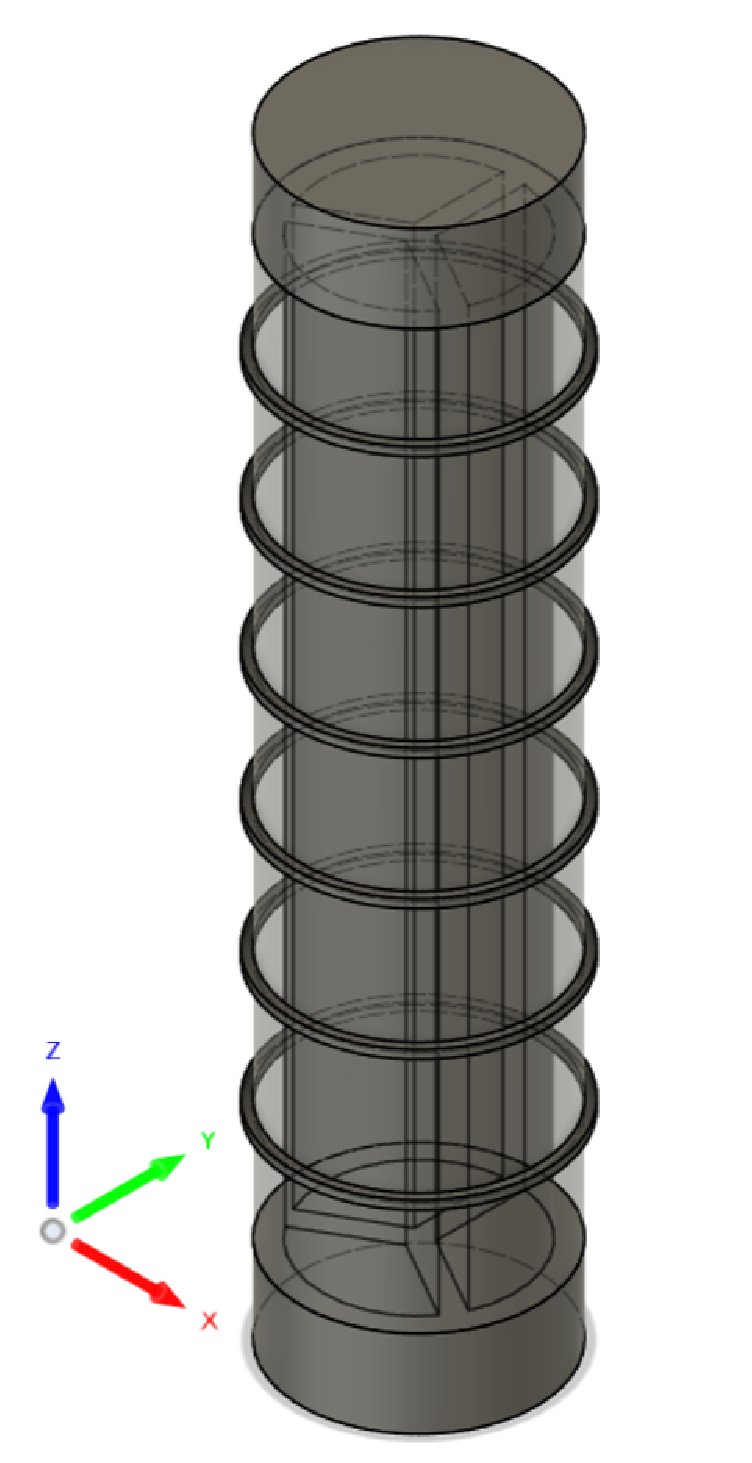
\includegraphics[height=38mm]{figures/actuatorSTL.eps}
  \hspace{5mm}
  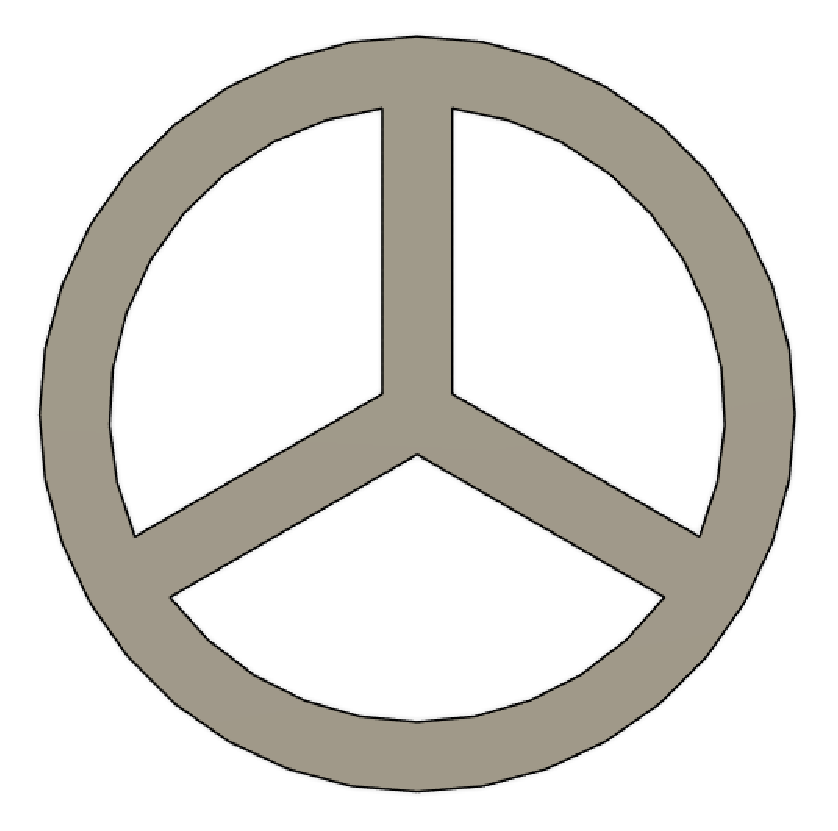
\includegraphics[height=30mm, angle=180]{figures/crossSection.eps}
  \vspace*{-2mm}
  \caption{Geometry of the soft pneumatic actuator. (Left) 3D view of the
  extruded silicone body. (Right) Cross-sectional view highlighting the
  three radially symmetric internal chambers and the central converging
  walls.}
  \label{fig:inchworm-geometry}
\end{figure}

\subsection{Finite-Element Optimization}

The primary objective of the structural optimization process was to minimize
the actuation pressure required to achieve a $180^\circ$ bending angle. To
evaluate the influence of the various design parameters on this objective,
Finite Element Method (FEM) simulations were conducted using COMSOL
Multiphysics, maintaining a constant length-to-diameter aspect ratio. The
elastomeric body (EcoFlex 00-30) was defined using the Yeoh hyperelastic
material model (incompressible)~\cite{Xavier2021Finite}, whereas the
reinforcing fibers and end caps were modeled as linear elastic
materials~\cite{Mao2020Soft}. The set of material parameters used in the
simulation is summarized in Table~\ref{tab:inchworm-materials}. To simulate
pneumatic actuation, a uniform pressure boundary load was applied to the
internal chamber walls. Gravity was neglected in the simulation for the sake
of simplicity.

\begin{table}[tb]
 \caption{Material properties and constitutive models used in the FEM
 simulations of the inchworm actuator.}
 \label{tab:inchworm-materials}
 \centering
 \footnotesize
 \setlength{\tabcolsep}{3pt}
 \begin{tabular}{|c|c|c|c|}
  \hline
  Material & \makecell{Constitutive \\ Model} & Parameter & Value \\ \hline
  \multirow{3}{*}{EcoFlex 00-30} & \multirow{3}{*}{Yeoh} & $C_1$ & 12.7 kPa \\
   &  & $C_2$ & 423 Pa \\
   &  & $C_3$ & -1.46 Pa \\ \hline
   \multirow{3}{*}{EcoFlex 00-50} & \multirow{3}{*}{Yeoh} & $C_1$ & $1.9 \times 10^{-2}$ MPa \\
   &  & $C_2$ & $9 \times 10^{-4}$ MPa \\
   &  & $C_3$ & $-4.75 \times 10^{-6}$ MPa \\ \hline
  \multirow{2}{*}{Aramid Fibers} & \multirow{2}{*}{Linear Elastic} & $E$ & 31 GPa \\
   &  & $\nu$ & 0.36 \\ \hline
  \multirow{2}{*}{PEI} & \multirow{2}{*}{Linear Elastic} & $E$ & 2.9 GPa \\
   &  & $\nu$ & 0.39 \\ \hline
 \end{tabular}
\end{table}

To quantify the resulting deformation, the Cartesian coordinates of two
diametrically opposed points ($P_1(x_1, y_1, z_1)$ and $P_2(x_2, y_2, z_2)$)
located at the tip of the actuator within the bending plane were evaluated.
Because the base of the actuator is constrained in a horizontal orientation
with its primary axis initially vertical, the bending angle $\theta$ is
geometrically defined as:
\begin{equation}
	\theta = \arctan \left( \frac{z_2 - z_1}{\sqrt{(x_2 - x_1)^2 + (y_2 - y_1)^2}} \right)
	\label{eqn:inchworm-bending}
\end{equation}

The parametric analysis indicated that minimizing both the fiber spacing and
the outer wall thickness significantly reduced the required operating
pressure. Furthermore, strategies to mitigate the ballooning effect of the
active internal chamber were investigated, specifically by incorporating
radial fiber reinforcements and by using an elastomer with a higher elastic
modulus (EcoFlex 00-50) for the internal walls. Interestingly, suppressing
the ballooning effect did not reduce the three-chambered actuator's pressure
requirements, as the unpressurized chambers inherently act as a
strain-limiting layer during bending. The simulation results are shown in
Fig.~\ref{fig:inchworm-comsol}.

\begin{figure*}[tb]
 \centering
  \includegraphics[height=40mm]{figures/comsol.eps}
  \vspace*{-2mm}
  \caption{FEM simulation results characterizing the soft actuator.
  (a)~Simulated stress distribution. (b)~Effect of circumferential fiber
  spacing on bending angle when a single chamber is pressurized at 2~kPa.
  (c)~Effect of silicone wall thickness on bending angle when a single
  chamber is pressurized at 3~kPa. (d)~Bending performance comparison for 1
  and 2 pressurized chambers at 3~kPa across three designs: a baseline
  actuator (EcoFlex 00-30) with 3~mm spaced circumferential fibers, a
  dual-material actuator with EcoFlex 00-50 internal walls, and an actuator
  with additional radial fibers spaced at 3~mm.}
  \label{fig:inchworm-comsol}
\end{figure*}
